\documentclass[11pt]{article}

% Change "review" to "final" to generate the final (sometimes called camera-ready) version.
% Change to "preprint" to generate a non-anonymous version with page numbers.
\usepackage[review]{acl}

% Standard package includes
\usepackage{times}
\usepackage{latexsym}
\usepackage[T1]{fontenc}
\usepackage[utf8]{inputenc}
\usepackage{microtype}
\usepackage{inconsolata}
\usepackage{graphicx}
\usepackage{amsmath}
\usepackage{amssymb}
\usepackage{xspace}
\usepackage{xcolor}

\newcommand{\model}{ProjectCraft\xspace}

\definecolor{darkgreen}{RGB}{0,100,0}

\newcommand{\nn}[1]{\textcolor{darkgreen}{TODO(Daniel): #1}}
\begin{document}

\section{Introduction}

Curating learning assignments is a crucial step in practice-oriented education, especially when the goal is to help learners develop practical skills.
A well-orchestrated assignment turns abstract learning objectives into concrete learner actions: learners practice by working through meaningful project tasks, making design decisions, and producing artifacts that can be inspected and evaluated~\cite{blumenfeld1991motivating,barron1998doing}.
However, crafting such assignments is non-trivial and time-consuming for teachers, because it requires the joint design of tasks, supporting materials, scaffolding, and evaluation criteria.
This motivates the need to explore automated methods for designing learning assignments while preserving meaningful learner work.

As shown in Figure~\ref{fig:demo}, designing such assignments requires preparing resources for both learners and instructors.
For learners, project materials define the concrete working context, including starter files, task instructions, requirements, resources, and expected deliverables.
For instructors, instructional procedures specify how the assignment should be taught, supported, and evaluated, including learning objectives, scaffolding strategies, checkpoints, assessment criteria, and feedback mechanisms.
These two sides must be designed jointly: materials for learners determine what work learners can perform, while guidance for instructors determines what that work is meant to teach and how progress should be assessed.

\begin{figure}[t]
    \centering
    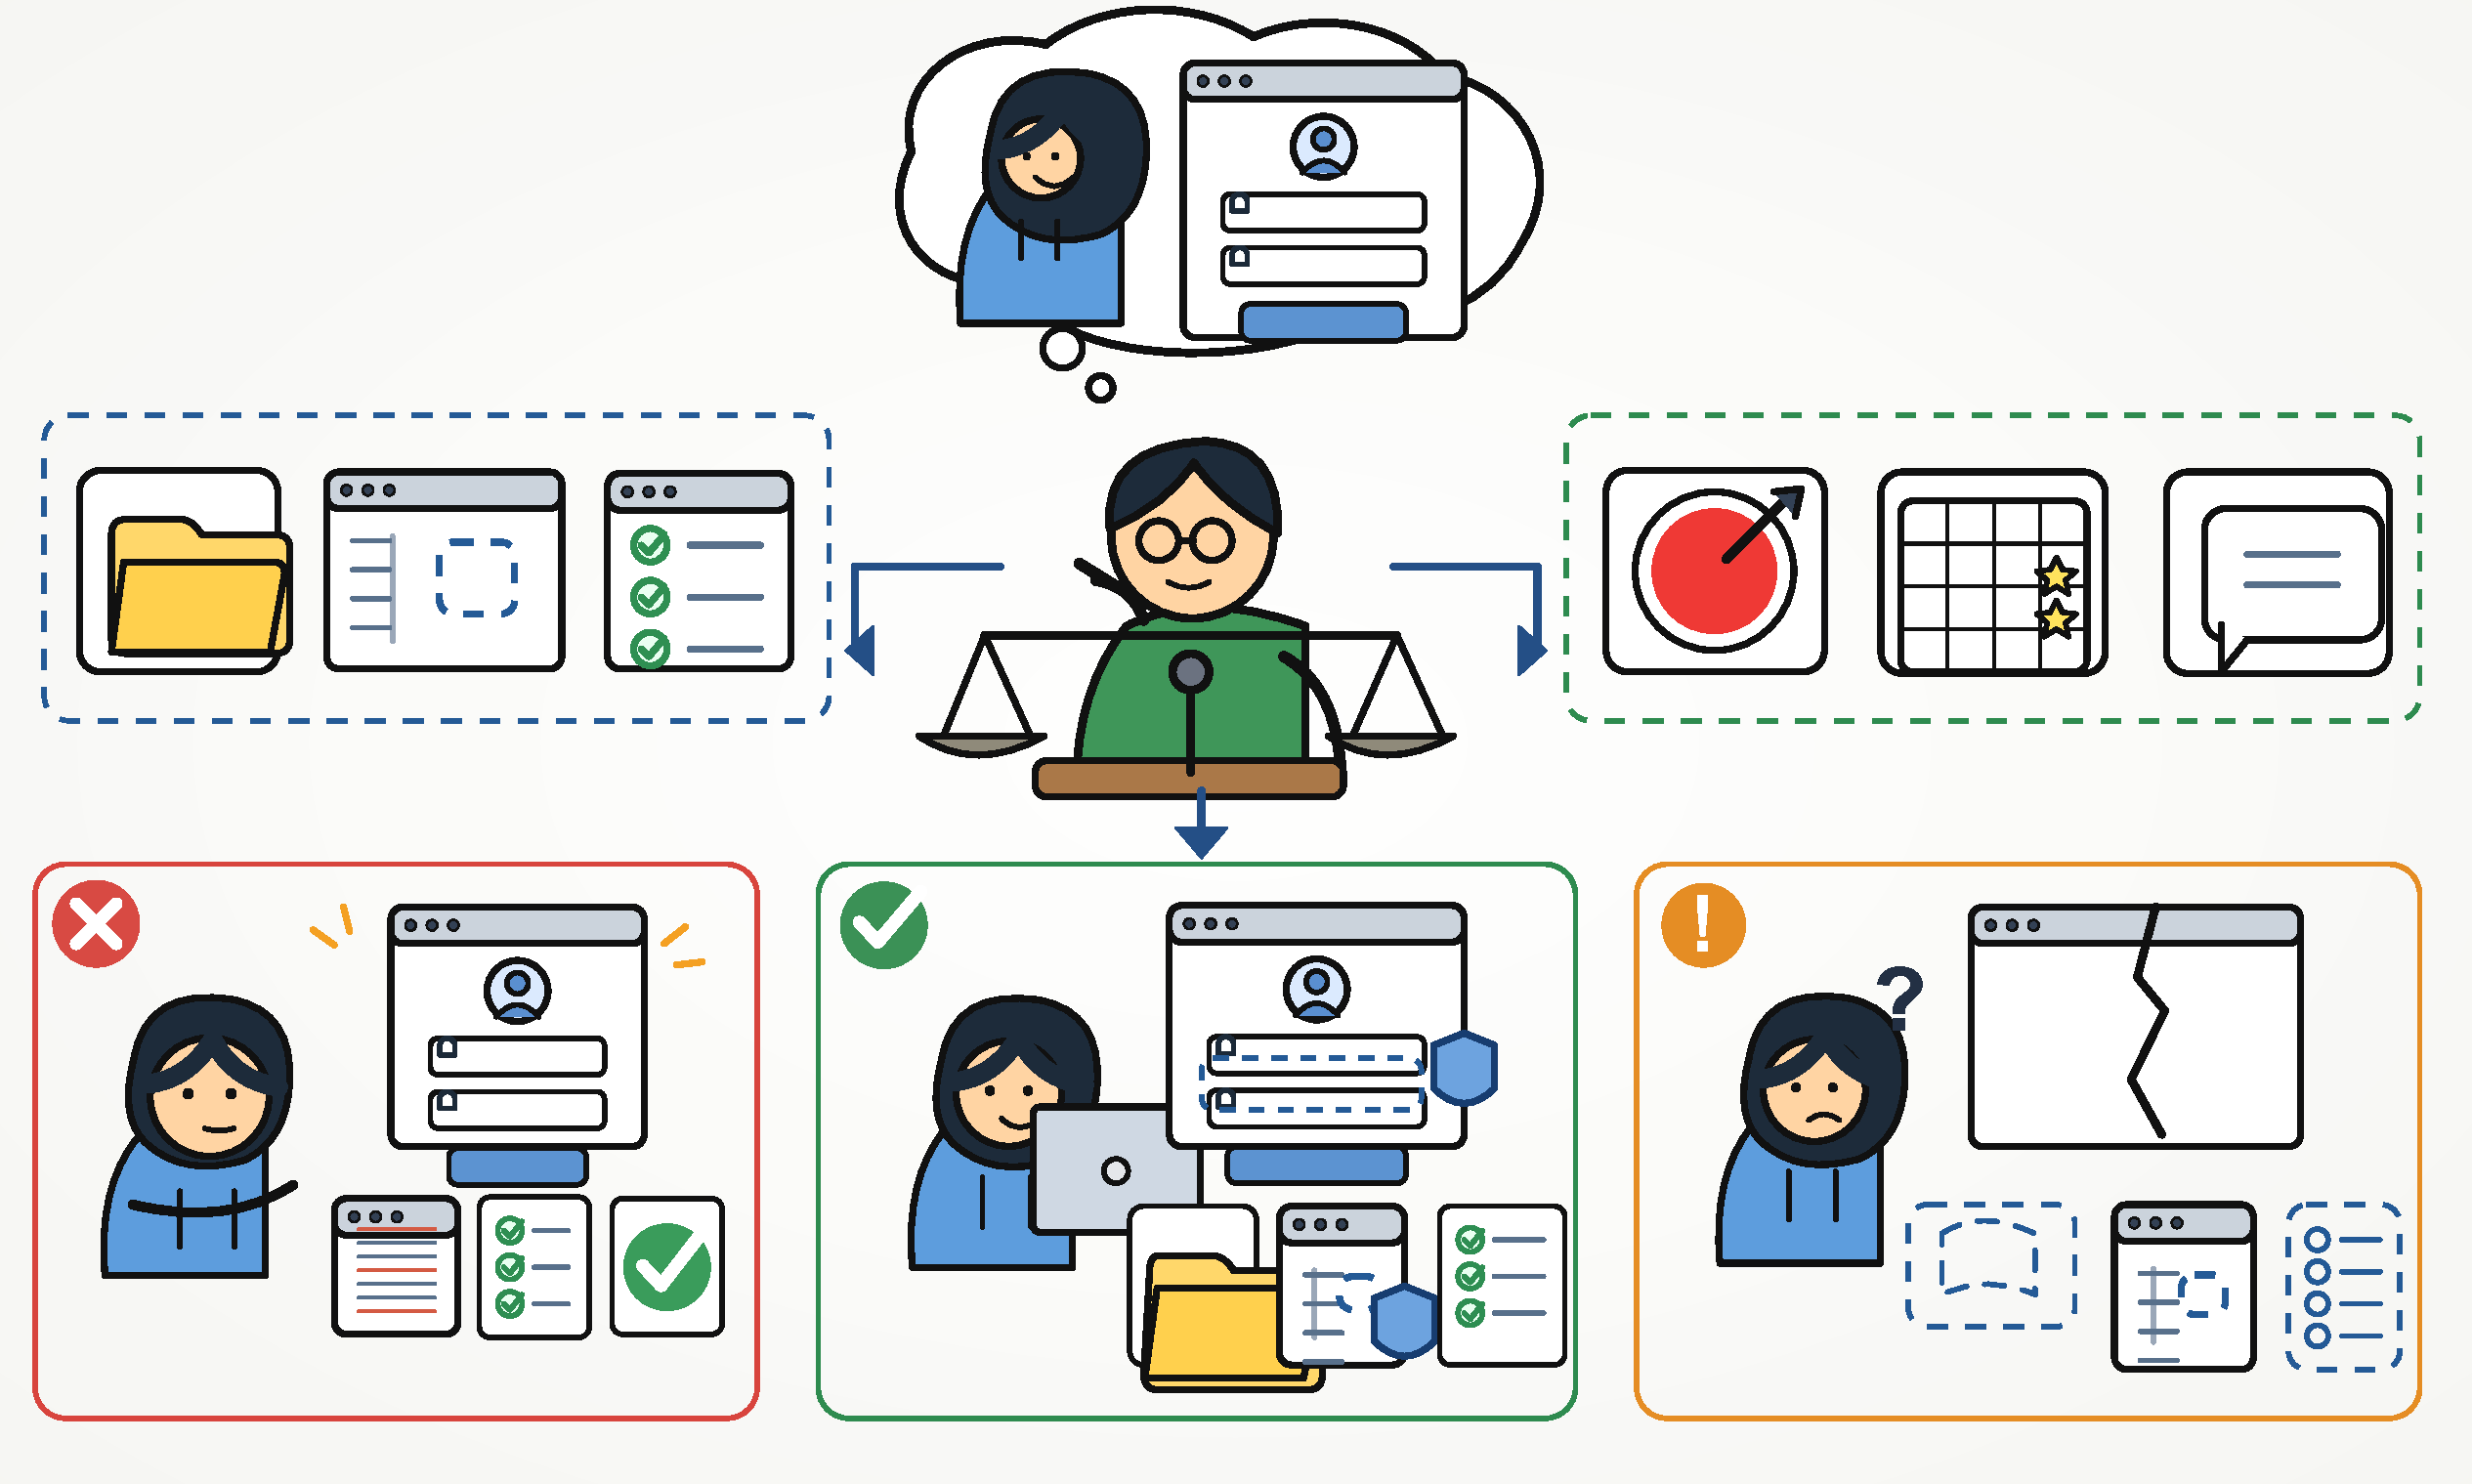
\includegraphics[width=\linewidth]{figures/demo-replica.pdf}
    \caption{Practice-assignment design requires coordinating learner-facing project materials with instructor-facing guidance so that the resulting assignment is executable while preserving meaningful learner-owned work.}
    \label{fig:demo}
\end{figure}

The difficulty is not only that these materials are numerous, but that they must remain coherent with one another.
The materials for learners must provide enough structure for students to make progress, while leaving open the parts of the task where learning should occur.
At the same time, the guidance for instructors must make clear why those parts are left open, how learners should be supported, and how their work should be assessed.
This makes assignment design both an engineering and a pedagogical problem: the system must decide what to build, what to scaffold, and what to leave for the learner.
These decisions interact: changing the project goal can change the required scaffolding, and changing the scaffolding can change what counts as meaningful learner work.


Existing LLM systems address parts of this engineering-pedagogical problem, but not the full assignment-design process.
Repository-level agents can generate and modify runnable code-bases~\cite{qian2023chatdev,hong2023metagpt,yang2024sweagent,wang2024openhands,zhang2024codeagent,shi2025autop2c}.
However, they are built to complete software artifacts, whereas a learning assignment must preserve selected work for the learner to perform.
In contrast, educational AI systems generate instructional content or support learning interactions, such as slides, question answering, textbooks, tutoring, scaffolding, and classroom simulation~\cite{zheng2025pptagent,zheng2026deeppresenter,shao2024storm,sharma2025pustakai,wang2024lessonplanner,zhang2024simclass,jang2026medtutor,cohn2026edf,deriyeva2026script,gao2024sinkt}.
These systems support instruction around a task, but typically do not generate a complete, aligned practice assignment.
Together, these gaps leave open a problem: how to turn a learner's goals into a complete, aligned practice assignment with meaningful learner work.


We propose \model, a framework for generating complete, aligned practice assignments from learner intent.
In this work, we realize these assignments as runnable training repositories tailored to individual learners.
\model first turns the learner's goals into an assignment plan that specifies the project materials, instructional procedures, target skills, scaffolding, and learner-owned work.
It then generates the corresponding repository components, including task instructions, starter files, scaffolds, tests, and validation behavior.
By coordinating materials for learners with guidance for instructors, \model aims to preserve meaningful learner work while scaling the creation of practice-oriented assignments.



\smallskip
\noindent In summary, our contributions are:
\begin{list}{$\bullet$}{%
    \setlength{\leftmargin}{1em}
    \setlength{\labelwidth}{0.5em}
    \setlength{\labelsep}{0.3em}
    \setlength{\itemsep}{0.2em}
    \setlength{\topsep}{0.2em}
    \setlength{\parsep}{0pt}
}
    \item We formulate practice-assignment generation as the task of transforming learner intent into complete, aligned assignments that coordinate project materials for learners, instructional guidance for instructors, and meaningful learner work.
    \item We introduce \model, a human-in-the-loop generation framework that coordinates project materials, instructional guidance, learner-aware scaffolding, repository construction, and validation to produce runnable training repositories with appropriate learner-owned work.
    \item We evaluate \model against direct generation baselines using both engineering and pedagogical criteria, showing improvements in repository validity, assignment alignment, and learner-work preservation.
\end{list}

\section{Related Work}

\subsection{Repository-Level Code Generation}

Recent LLM-based software engineering systems increasingly target repository-level generation.
ChatDev~\cite{qian2023chatdev} and MetaGPT~\cite{hong2023metagpt} decompose development into role-based multi-agent workflows, while SWE-agent~\cite{yang2024sweagent}, OpenHands~\cite{wang2024openhands}, and CodeAgent~\cite{zhang2024codeagent} equip agents with tools for navigating, editing, and testing real codebases.
AutoP2C~\cite{shi2025autop2c} is closest to our setting, transforming academic papers into executable repositories.
Yet these systems optimize for executable completeness: implementation gaps are defects to eliminate.
A2P targets a different objective, where the repository must run while preserving deliberately chosen gaps as learner-owned work.

\subsection{Educational Content Generation}

LLMs have also been used to generate educational materials and learning interactions.
Systems such as PPTAgent~\cite{zheng2025pptagent}, DeepPresenter~\cite{zheng2026deeppresenter}, STORM~\cite{shao2024storm}, and PustakAI~\cite{sharma2025pustakai} produce instructional artifacts such as slides, articles, and textbooks, while LessonPlanner~\cite{wang2024lessonplanner} supports pedagogy-driven lesson planning.
Tutoring systems take a complementary approach: SimClass~\cite{zhang2024simclass} simulates classroom interaction, MedTutor~\cite{jang2026medtutor} supports case-based medical education, and EDF~\cite{cohn2026edf} implements theory-driven adaptive scaffolding.
Co-design work with K-12 educators further shows that project design is a major pain point where LLM support is desired~\cite{lee2025codesigning}.
However, these systems primarily generate instructional content or interactions around learning.
A2P instead generates the executable setting in which learning occurs: source concepts are instantiated as files, tests, tasks, scaffolds, and learner-owned implementation gaps.

\subsection{Scaffolding and Learner Modeling}

Scaffolding theory explains why incompletion in a learning repository must be controlled rather than arbitrary.
Vygotsky's zone of proximal development~\cite{vygotsky1978} and Wood et al.'s scaffolding framework~\cite{wood1976scaffolding} establish that effective instruction targets work learners cannot yet complete independently but can complete with support.
Cognitive load theory~\cite{sweller1988cognitive} provides the complementary constraint: excessive unsupported complexity prevents learning, while productive failure~\cite{kapur2008productive} and desirable difficulties~\cite{bjork2011desirable} show that appropriately challenging struggle can improve learning.
This balance is central to PBL, where authentic artifacts require structured support rather than minimal guidance~\cite{kirschner2006minimal,hmelosilver2007scaffolding,krajcik2014pbl}.
A2P operationalizes this balance as a repository-generation problem: deciding which components should be complete, scaffolded, or left as learner-owned implementation gaps.

On the computational side, learner modeling has evolved from Bayesian Knowledge Tracing~\cite{corbett1995knowledge} through deep knowledge tracing~\cite{piech2015deep} to LLM-augmented approaches such as SINKT~\cite{gao2024sinkt}, which uses LLM-encoded concept semantics for inductive knowledge tracing.
These systems model learners for \emph{runtime} adaptation---selecting or sequencing existing content.
A2P instead uses a one-shot learner profile to condition \emph{generation}, deciding what to scaffold, what to leave as productive struggle~\cite{kapur2008productive}, and what to omit as noise \emph{before} the project exists.

\section{\model: Practice Assignment Generation}

To support practice-assignment generation, we propose \model, a planning framework that transforms learner goals and source artifacts into runnable training repositories.
\model treats an assignment not as a single generated document or codebase, but as a coordinated design over learning goals, project materials, instructional guidance, task ownership, scaffolding, and validation.
This formulation is guided by two requirements.
First, the generated assignment must be complete enough to support execution: learners need concrete files, instructions, milestones, support resources, and criteria for checking progress.
Second, the assignment must remain incomplete in the right places: work that is central to the target skill should be preserved for the learner rather than solved by the system.
\model addresses these requirements by representing assignments as coupled design components and instantiating them through a phase-gated workflow.

\subsection{Assignment Representation}

\model represents a practice assignment as five aligned decisions: what the learner should practice, what materials instantiate that practice, how support should be provided, what work should remain learner-owned, and how progress should be validated.
These decisions correspond to \textit{learning intent}, \textit{project materials}, \textit{instructional guidance}, \textit{task ownership}, and \textit{validation}.
Together, they specify the target skill and deliverable, the concrete files and documents learners will use, the scaffolds and assessment criteria that guide instruction, the responsibilities of learners and supporting roles, and the tests or rubrics used to check completion.

The key property of this representation is alignment.
A change in learner proficiency can require different scaffolds, milestones, and learner-owned gaps; a change in validation criteria can alter what starter files or instructions are needed.
\model therefore uses this representation as a planning constraint: later artifacts are generated only after these assignment-level decisions have been made consistent with one another.

\subsection{Phase-Gated Workflow}

Figure~\ref{fig:method-overview} illustrates the end-to-end workflow of \model.
To show how learner goals become an executable practice assignment, we first summarize the full process before describing the main design mechanisms.
The workflow consists of five phases: \textit{Clarify}, \textit{Frame}, \textit{Orchestrate}, \textit{Materialize}, and \textit{Instantiate}.
Each phase stabilizes one layer of assignment design before later phases generate more detailed artifacts.

\begin{figure}[t]
    \centering
    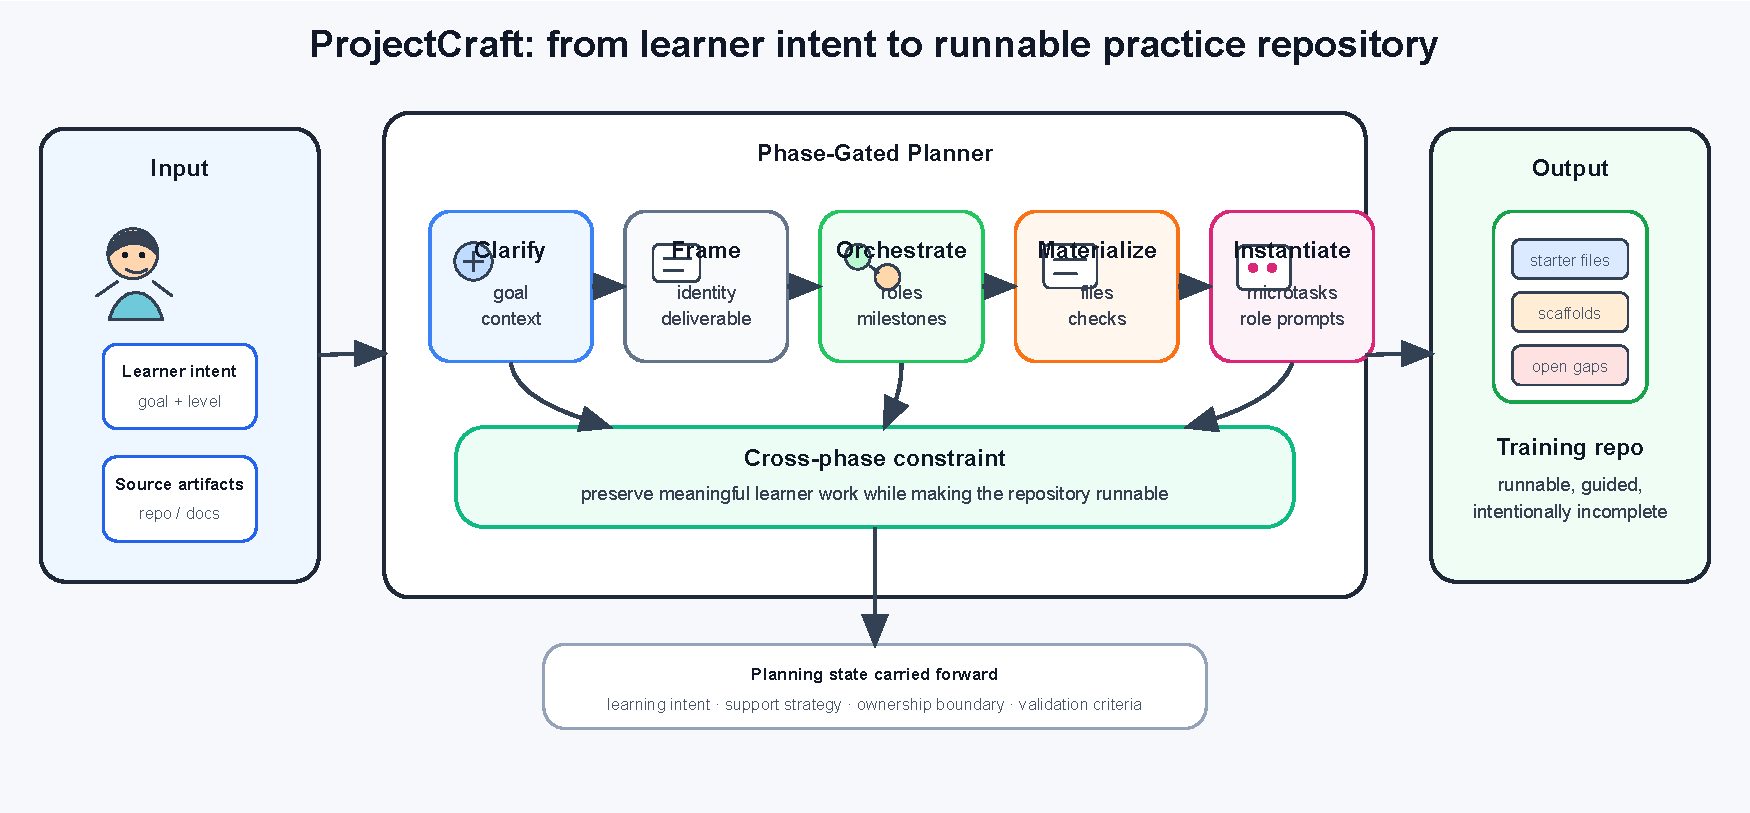
\includegraphics[width=\linewidth]{figures/method-overview.pdf}
    \caption{The phase-gated workflow of \model. The system progressively stabilizes learner intent, assignment identity, collaboration structure, concrete materials, and execution-ready microtasks while maintaining a cross-phase constraint that meaningful learner work remains learner-owned.}
    \label{fig:method-overview}
\end{figure}

In the \textit{Clarify} phase, \model interprets the learner's goal and available context.
Learning goals may be stated at different levels of specificity, ranging from a broad topic or source repository to a concrete project deliverable.
\model identifies the intended learning outcome, the available source context, and the learner's proficiency so that subsequent decisions can be calibrated to the learner rather than to a generic project template.
The output is a stabilized learning intent that anchors the remaining workflow.

In the \textit{Frame} phase, \model turns the stabilized intent into an assignment identity.
This includes the project goal, final deliverable, title, description, and topical tags.
The purpose of this phase is to make the assignment legible before detailed tasks or files are produced: the system first decides what the learner is working toward, then decides how that work should be organized.

In the \textit{Orchestrate} phase, \model designs the collaboration pattern for the assignment.
It creates milestones, introduces the roles needed to support the learner, and determines how responsibility should be distributed across learner work, instructor oversight, AI assistance, and optional scene interaction.
Every assignment includes a learner role and an instructor role.
Depending on the assignment type, \model may also introduce AI collaborators for implementation support, checking, research, or scaffolding, and scene actors for role-play settings such as interviews, negotiation, or communication practice.

In the \textit{Materialize} phase, \model generates the concrete resources needed for the assignment.
These include starter files, configuration files, fixtures, examples, learner documents, scaffolds, and validation resources.
This phase turns the assignment from a plan into a workspace context in which the learner can act.

In the \textit{Instantiate} phase, \model turns each milestone into execution-ready microtasks.
Each microtask specifies its goal, responsible role, participants, expected output, and role-specific guidance for execution.
The resulting assignment can then be reviewed by the learner and passed to the workspace execution phase, where the learner, instructor, AI collaborators, and optional scene actors interact around the generated tasks.

\subsection{Learning-Preserving Task Synthesis}

A key challenge in task synthesis is to make the generated project executable while preserving the learner work that carries the intended practice.
\model therefore distinguishes between core learning work and auxiliary work.
Core learning work includes decisions, implementations, analyses, or communications that directly exercise the target skill.
Auxiliary work includes setup, boilerplate, repetitive configuration, mechanical glue code, or contextual preparation that is necessary for execution but not central to the learning objective.
\model preserves core learning work for the learner, while assigning auxiliary work to system-generated materials or AI collaborators when doing so helps the learner focus on the intended skill.

Learner proficiency controls how this ownership boundary is drawn and how it appears in the generated assignment.
For beginners, \model uses smaller milestones, denser scaffolding, more explicit instructions, and greater system support for setup and navigation.
For intermediate learners, the system shares responsibility between learner work and AI assistance, preserving meaningful design and implementation choices while providing targeted support.
For advanced learners, \model leaves more architectural decisions, implementation gaps, and validation reasoning to the learner, while using AI roles mainly for feedback, review, and verification.
These choices are reflected in milestone granularity, task descriptions, starter-file gaps, scaffolds, and validation criteria, so learner adaptation changes the structure of the assignment rather than only the wording of the instructions.

\subsection{Repository Realization}

Repository realization turns the planned assignment into a concrete training repository.
Using the learning intent, support strategy, ownership boundary, and validation criteria determined in earlier phases, \model generates the materials needed for practice: starter files, requirements, examples, documents, scaffolds, and checks.
These materials give learners a concrete context in which to work, while the associated guidance records how that work should be supported and evaluated.

The resulting repository is designed to be runnable but not complete.
Starter materials provide the initial code, documents, and task context needed to begin the assignment.
When a source artifact such as a GitHub repository is available, \model uses it to derive realistic starter files, constraints, examples, and validation checks.
At the same time, \model leaves intentional gaps where learners should make decisions, implement functionality, conduct analysis, or produce communicative artifacts.
These gaps are chosen to exercise the target skill, so the repository remains a learning environment rather than a completed solution.
\model then generates tests, rubrics, or milestone checks based on the work the learner is expected to complete.

\section{Experiment}

In this section, we evaluate whether \model can support the generation of practice assignments from learner intent.
As discussed in the previous sections, this setting differs from conventional repository generation because the output is not only expected to be executable, but also to function as a learning environment with aligned materials, scaffolding, validation, and learner-owned work.
We therefore organize our evaluation around four research questions:
\begin{list}{$\bullet$}{%
    \setlength{\leftmargin}{1em}
    \setlength{\labelwidth}{0.5em}
    \setlength{\labelsep}{0.3em}
    \setlength{\itemsep}{0.2em}
    \setlength{\topsep}{0.2em}
    \setlength{\parsep}{0pt}
}
    \item \textbf{RQ1: Repository validity.} Can \model generate complete and executable practice-assignment repositories?
    \item \textbf{RQ2: Pedagogical alignment.} Are the generated repositories aligned with the learner's intent across project materials, scaffolding, validation, and instructor guidance?
    \item \textbf{RQ3: Learner-owned work preservation.} Does \model preserve meaningful learner-owned work while providing sufficient support for the assignment to be actionable?
    \item \textbf{RQ4: Phase-gated planning.} How much does the phase-gated workflow contribute compared with direct generation?
\end{list}


\bibliography{custom}

\end{document}
